%\documentclass{article}
%\usepackage[utf8]{inputenc}
%\title{test}
%\author{paolo.dini }
%\date{June 2017}
%\begin{document}
%\maketitle
%\section{Introduction}
%\end{document}

%===================================================
%================== DOCUMENT CLASS
%===================================================
\documentclass[runningheads,11pt,a4paper,english,llncs]{Misc/llncs}

%===================================================
%================== PACKAGES
%===================================================
%------------------------------------------------------------------------
% TeX and LaTeX macros
%------------------------------------------------------------------------
%
% In math formulas we use italic instead of mathitalic
%
\makeatletter
% ~ gives a \; space in math mode
\def~{\ifmmode\;\else\penalty\@M\ \fi}
%  Italic in mathematical formulas
\def\@setmcodes#1#2#3{{\count0=#1 \count1=#3
  \loop \global\mathcode\count0=\count1 \ifnum \count0<#2
  \advance\count0 by1 \advance\count1 by1 \repeat}}
\DeclareSymbolFont{italic}{OT1}{\rmdefault}{m}{it}
\let\mathit\undefined
\DeclareSymbolFontAlphabet{\mathit}{italic}
\edef\@tempa{\hexnumber@\symitalic}
\@setmcodes{`A}{`Z}{"7\@tempa41}
\@setmcodes{`a}{`z}{"7\@tempa61}
\makeatother
%
% \begin{asm} ... \end{asm}
%
\newdimen\asmindent     
\asmindent=\parindent
\newcount\asmi
\def\inc{\global\advance\asmi by 1}
\def\dec{\global\advance\asmi by-1}
\def\nl{{}$\par\hangindent\asmi em
  \noindent\kern\asmi em\ignorespaces$} 
\def\asmskip{{}$\par\smallskip\hangindent\asmi em
  \noindent\kern\asmi em\ignorespaces$} 
\def\asm{\global\asmi=0 
%%%%%%%%%%%%%% added by Paolo:
\parskip=0pt
%%%%%%%%%%%%%%%%%%%%%%%%%%%%%
 \def\+{\inc\nl}
 \def\-{\dec\nl}
 \def\\{\nl}
 \begin{trivlist}
 \item[]\leftskip=\asmindent\relax$}
\def\endasm{$
\end{trivlist}}
%\mathindent=\asmindent
%
% \begin{asmarray}
%    f(s_1) & := t_1 \\
%    f(s_2) & := t_2 
% \end{asmarray}
%
\def\asmarray{\begin{array}[t]{@{}l@{\;}l@{\;}l@{}}}
\def\endasmarray{\end{array}}
%
%
%
\def\asmcomment#1{\quad\hbox{// #1}}
%
%  \begin{subasm} ... \end{subasm}
%
\newcount\asmii
\def\subasm{\vtop\bgroup\asmii=0\normalbaselines
 \def\nl##1{$\egroup\advance\asmii by##1\relax\hbox\bgroup\hskip\asmii em$}
 \def\\{\nl{0}}
 \def\+{\nl{1}}
 \def\-{\nl{-1}}
 \hbox\bgroup\hskip\asmii em$}
\def\endsubasm{$\egroup\egroup}
%
% Keywords in ASM code
%
\def\ASM#1{\hbox{\sc#1}}        % rule names and macros
\def\ASMIND#1{\ASM{#1}\index{#1@{\sc#1}}}
\def\AWAIT   {\mathrel{\mathbf{await}}}
\def\AND     {\mathrel{\mathbf{and}}}
\def\CASE    {\mathrel{\mathbf{case}}}
\def\CHOOSE  {\mathrel{\mathbf{choose}}}
\def\CREATE  {\mathrel{\mathbf{create}}}
\def\NEW  {\mathrel{\mathbf{new}}}
\def\DO      {\mathrel{\mathbf{do}}}
\def\ELSE    {\mathrel{\mathbf{else}}}
\def\ELSEIF  {\mathrel{\mathbf{elseif}}}
\def\FORALL  {\mathrel{\mathbf{forall}}}
\def\FORSOME  {\mathrel{\mathbf{forsome}}}
\def\FOREACH  {\mathrel{\mathbf{foreach}}}
\def\IF      {\mathrel{\mathbf{if}}}
\def\IMPORT  {\mathrel{\mathbf{import}}}
\def\IN      {\mathrel{\mathbf{in}}}
\def\LET     {\mathrel{\mathbf{let}}}
\def\SELF    {\mathrel{\mathbf{self}}}
\def\MATCH    {\mathrel{\textbf{match}}}
\def\NOT     {\mathrel{\mathbf{not}}}
\def\OF      {\mathrel{\mathbf{of}}}
\def\OR      {\mathrel{\mathbf{or}}}
\def\PAR     {\mathrel{\mathbf{par}}}
\def\SEQ     {\mathrel{\mathbf{seq}}}
\def\SKIP    {\mathrel{\mathbf{skip}}}
\def\THEN    {\mathrel{\mathbf{then}}}
\def\WHERE   {\mathrel{\mathbf{where}}}
\def\WHILE   {\mathrel{\mathbf{while}}}
\def\UNDEF   {\mathrel{\mathbf{undef}}}
\def\UNTIL   {\mathrel{\mathbf{until}}}
\def\WHEN   {\mathrel{\mathbf{when}}}
\def\WITH    {\mathrel{\mathbf{with}}}
\def\STEP    {\mathrel{\mathbf{step}}}
\def\STEPWISE    {\mathrel{\mathbf{stepwise}}}
\def\SEQ    {\mathrel{\mathbf{seq}}}
\def\RESULT  {\mathrel{\mathbf{result}}}
\def\CALL  {\mathrel{\mathbf{Call}}}
\def\LOCAL    {\mathrel{\mathbf{local}}}
\def\ADDGUARD {\mathrel{\mathbf{addGuard}}}
\def\ADDUPD   {\mathrel{\mathbf{addUpd}}}
\def\ADDRULE  {\mathrel{\mathbf{addRule}}}
\def\MINUSRULE  {\mathrel{\mathbf{minusRule}}}
\def\TO      {\mathrel{\mathbf{to}}}
%
% Including figures
%
\def\includefig#1#2{\centering\medskip
  \includegraphics[scale=#1]{fig/#2}
  \medskip}
%
% References to paragraphs in the ECMA standard for C#
%
\def\ecma#1{\cite[\S#1]{ecma334}}
%
%  Environments for definitions and theorems
%
%\theorembodyfont{\rm}
%\newtheorem{definition}[subsection]{Definition}
%\newtheorem{lemma}[subsection]{Lemma}
%\newtheorem{theorem}[subsection]{Theorem}
%\newtheorem{proposition}[subsection]{Proposition}
%\newtheorem{corollary}[subsection]{Corollary}
%\newtheorem{example}[subsection]{Example}
%\newtheorem{remark}[subsection]{Remark}
%\newtheorem{constraint}[subsection]{Constraint}
\def\proof{\trivlist\item[]{\bf Proof.}}
\def\endproof{$\Box$\endtrivlist}
%
% enumerate and itemize (smaller skips) from "latex.ltx"
%
\makeatletter
\def\enumerate{%
  \ifnum \@enumdepth >\thr@@\@toodeep\else
    \advance\@enumdepth\@ne
    \edef\@enumctr{enum\romannumeral\the\@enumdepth}%
      \expandafter
      \list
        \csname label\@enumctr\endcsname
        {\usecounter\@enumctr\def\makelabel##1{\hss\llap{##1}}
         \itemsep 0pt\parskip 0pt\parsep 0pt\topsep\smallskipamount}%
  \fi}
\def\itemize{%
  \ifnum \@itemdepth >\thr@@\@toodeep\else
    \advance\@itemdepth\@ne
    \edef\@itemitem{labelitem\romannumeral\the\@itemdepth}%
    \expandafter
    \list
      \csname\@itemitem\endcsname
      {\def\makelabel##1{\hss\llap{##1}}
       \itemsep 0pt\parskip 0pt\parsep 0pt\topsep\smallskipamount}%
  \fi}
\makeatother
%
% items in itemize
%
\def\bull{\vrule height .9ex width .8ex depth -.1ex}
\def\labelitemi{\bull}
%
%
%
\def\cs#1{C\#$_{\mathcal{#1}}$}
\def\lang#1{L$_{\mathcal{#1}}$}
%
% Positions
%
\def\pos#1{{}^{#1}}
\def\termPos{\blacktriangleright}
\def\cursor{\pos{\termPos}}
%
%
%
\def\sup{\hbox{sup}}
\def\c#1{\texttt{#1}}           % code
\def\N#1{\textit{#1}}           % non terminal symbols
\def\T#1{\hbox{`\texttt{#1}'}}  % terminal symbols
\def\A#1{\hbox{\sc#1}}          % ASM rules
\def\D#1{#1}                    % dynamic functions
\def\U#1{#1}                    % universes
\def\C#1{#1}                    % constructors
\def\rdef{\equiv}
\def\lbr{\c{\char`\{}}
\def\rbr{\c{\char`\}}}
\def\mb{\hbox{::}}
\def\map#1#2{\textbf{Map from}~#1~\textbf{to}~#2}
\def\cat{\cdot}
\def\adots{\mathinner{\ldotp\ldotp}}
%
%
% macros.tex ends here

\usepackage{etex}
\reserveinserts{28}
\newcommand{\todo}[1]{
 \noindent{\newline \color{red}
 \framebox[\textwidth][t]{%
  \parbox[t]{0.9\textwidth}{\textcolor{red}{TODO: #1}}                                                                                     
}}}


%===================================================
%================== PACKAGES
%===================================================
\usepackage{graphicx}
\usepackage{acronym}
\usepackage{ifthen}
\usepackage{substr}
\usepackage{color}
\usepackage{fixltx2e}
\usepackage[left=2cm, top=2cm, right=2cm, bottom=2cm]{geometry}
%\usepackage{subfigure}
\usepackage{array,rotating}          
\usepackage{url}
%\usepackage{enumerate}
\usepackage[shortlabels]{enumitem}
\usepackage{epsfig}
\usepackage{colordvi}
\usepackage{makeidx}
\usepackage{index}
\usepackage[absolute]{textpos}
\setlength{\TPHorizModule}{\paperwidth}
\setlength{\TPVertModule}{\TPHorizModule}
\textblockorigin{-6mm}{0mm}
\usepackage[%
      breaklinks=true,%
      colorlinks=true,%           no frame around URL
      urlcolor=LINK_COLOR,%            no colors
      menucolor=LINK_COLOR,%           no colors
      linkcolor=LINK_COLOR,%           no colors
      pagecolor=LINK_COLOR,%           no colors
      bookmarks=true,%            tree-like TOC
      bookmarksopen=false,%       expanded when starting
      hyperfootnotes=true,%       no referencing of footnotes, does not compile
      citecolor=CITE_COLOR,%           black cites
      filecolor=black,%           black files%
      hyperindex=true,%
      hyperfigures=true%
]{hyperref}
\usepackage{bookmark}
\usepackage{booktabs}
\usepackage{dsfont}
\usepackage{wallpaper}
\usepackage{mathtools,cancel}
\usepackage{soul}
\usepackage{float}
\usepackage{setspace}
%\usepackage{morefloats}
%\usepackage{mdwlist}
\usepackage{amsmath,amssymb,amscd,diagrams,bm,amsfonts}
\let\proof\relax
\let\endproof\relax
\usepackage{amsthm}
\usepackage{tabularx, graphics, longtable}
%TIKZ
\usepackage{tikz}
\usepackage{tikz-cd}
\usetikzlibrary{trees,snakes}
\usetikzlibrary{arrows,automata}
\usetikzlibrary{matrix,arrows,positioning}
\usetikzlibrary{mindmap,backgrounds}
\usetikzlibrary{shapes}
\usepackage{verbatim} %for comment out some texts


%%%%%%%%%%%%%%%%%%%%%%%%%%%%%%%
%%%%%%%%%%%%%%%%%%%%% Egon's commands:
\usepackage{latexsym}
\ifx\pdfoutput\undefined
  \message{We are running LaTeX.} 
%PD  \usepackage[dvips]{graphicx}
%PD  \DeclareGraphicsExtensions{.eps}
%PD  \usepackage[hypertex,bookmarks=false]{hyperref}
\else
  \message{We are running PDFLaTeX.}
%PD  \usepackage[pdftex]{color}
%PD  \usepackage[pdftex]{graphicx}
%PD\DeclareGraphicsExtensions{.jpg,.pdf}
%PD  \DeclareGraphicsExtensions{.pdf}
%PD  \usepackage[pdftex,bookmarks=false]{hyperref}
%PD  \hypersetup{colorlinks={true},
%PD            linkcolor={blue},
%PD            citecolor={blue},
%PD            urlcolor={blue},
%PD            plainpages={false}
%PD  }
\fi
%%%%%%%%%%%%%%%%%%%%%%%%%%%%%%%
%%%%%%%%%%%%%%%%%%%%%%%%%%%%%%%


%===================================================
%================== COLOURS
%==================================================

\definecolor{green}{rgb}{0,0.6,0} 
\definecolor{gray}{rgb}{0.6,0.6,0.6} 
\definecolor{red}{rgb}{1,0,0} 
\definecolor{blue}{rgb}{0,0,1} 
\definecolor{purple}{rgb}{0.5,0,0.5} 
\definecolor{yellow}{rgb}{0.25,0.25,0} 
\definecolor{turquoise}{rgb}{0,0.5,0.5}
\definecolor{brown}{rgb}{0.6,0.2,0.1}

\definecolor{LINK_COLOR}{rgb}{0,0,0.7}
\definecolor{CITE_COLOR}{rgb}{0,0.5,0}
\definecolor{lightblue}{rgb}{0,0,1}
\definecolor{light-gray}{gray}{0.95}
\def\red#1{\textcolor[rgb]{1.0,0.0,0.0}{#1}}
\def\green#1{\textcolor[rgb]{0.0,0.8,0.1}{#1}}
\def\blue#1{\textcolor[rgb]{0.0,0.0,1.0}{#1}}

%===================================================
%================== LAYOUT
%===================================================
\parindent=0cm
%\setlength{\parskip}{1.0\baselineskip plus 0.5ex minus 0.2ex}
\abovecaptionskip=0cm
\hyphenpenalty=5000
\tolerance=1000 
\floatsep=1in
\allowdisplaybreaks
\def \constzeroindent {0cm}
\def \constfirstindent {0.5cm}
\def \constsecondindent {1cm}
\newenvironment{mycustomindent}[1]
{\setlength{\parindent}{#1}}
{\setlength{\parindent}{\constzeroindent}}
\newcommand{
	\firstindent}[1]{
	\begin{mycustomindent}{\constfirstindent}
	\begin{tabular}{@{}p{12cm}@{}}
	#1 \\
	\end{tabular}
	\end{mycustomindent}
}
\newcommand{
	\secondindent}[1]{
	\begin{mycustomindent}{\constsecondindent}
	\begin{tabular}{@{}p{12cm}@{}}
	#1 \\
	\end{tabular}
	\end{mycustomindent}
}
\newenvironment{packed_item1}{
\begin{itemize}[topsep=0pt, partopsep=0pt]
  \setlength{\itemsep}{5pt}
  \setlength{\parskip}{0pt}
  \setlength{\parsep}{0pt}
}{\end{itemize}}
\newenvironment{packed_item2}{
\begin{itemize}[topsep=0pt, partopsep=0pt]
  \setlength{\itemsep}{0pt}
  \setlength{\parskip}{0pt}
  \setlength{\parsep}{0pt}
}{\end{itemize}}
\newenvironment{packed_enumerate}{
\begin{enumerate}[topsep=0pt, partopsep=0pt]
  \setlength{\itemsep}{5pt}
  \setlength{\parskip}{0pt}
  \setlength{\parsep}{0pt}
}{\end{enumerate}}
% The following commands are to get rid of the extra space around section and subsection titles:
% Save the class definition of \subparagraph:
\let\llncssubparagraph\subparagraph
% Provide a definition to \subparagraph to keep titlesec happy:
\let\subparagraph\paragraph
\usepackage[compact]{titlesec}
\usepackage{dblfloatfix,caption,subcaption}
\titlespacing{\section}{0pt}{12pt}{*0}
\titlespacing{\subsection}{0pt}{6pt}{0pt}
\titlespacing{\subsubsection}{0pt}{6pt}{0pt}
% Force section numbering to follow chapter numbering:
\usepackage{chngcntr}
\counterwithin{section}{chapter}
\counterwithin{figure}{chapter}
%\counterwithin{theorem}{chapter}
%\counterwithin{lemma}{chapter}
%\counterwithin{definition}{chapter}
%%%%%%%%%%%%%%%%%%%%%%%%%%%%
% Allow line breaks in long list of citations that would extend into the margin:
\usepackage{breakcites}
%%%%%%%%%%%%%%%%%%%%%%%%%%%%%%%%%%%%%%

\usepackage{pdfpages}
\pagestyle{headings}

\renewcommand{\rightmark}{INTERLACE Project (Grant no.~754494)}
\renewcommand{\leftmark}{D2.1}
\setcounter{tocdepth}{2}

\usepackage{tocloft}
\setlength\cftparskip{0pt}
\setlength\cftbeforechapskip{12pt}

\usepackage{abstract}
\renewcommand{\abstractnamefont}{\large \bfseries}
%\setlength{\abstitleskip}{-\absparindent}
\renewcommand{\abstractname}{Abstract}

\setlength{\parskip}{12pt}

\begin{document}
%===================================================
%================== TITLE
%===================================================

\thispagestyle{empty}
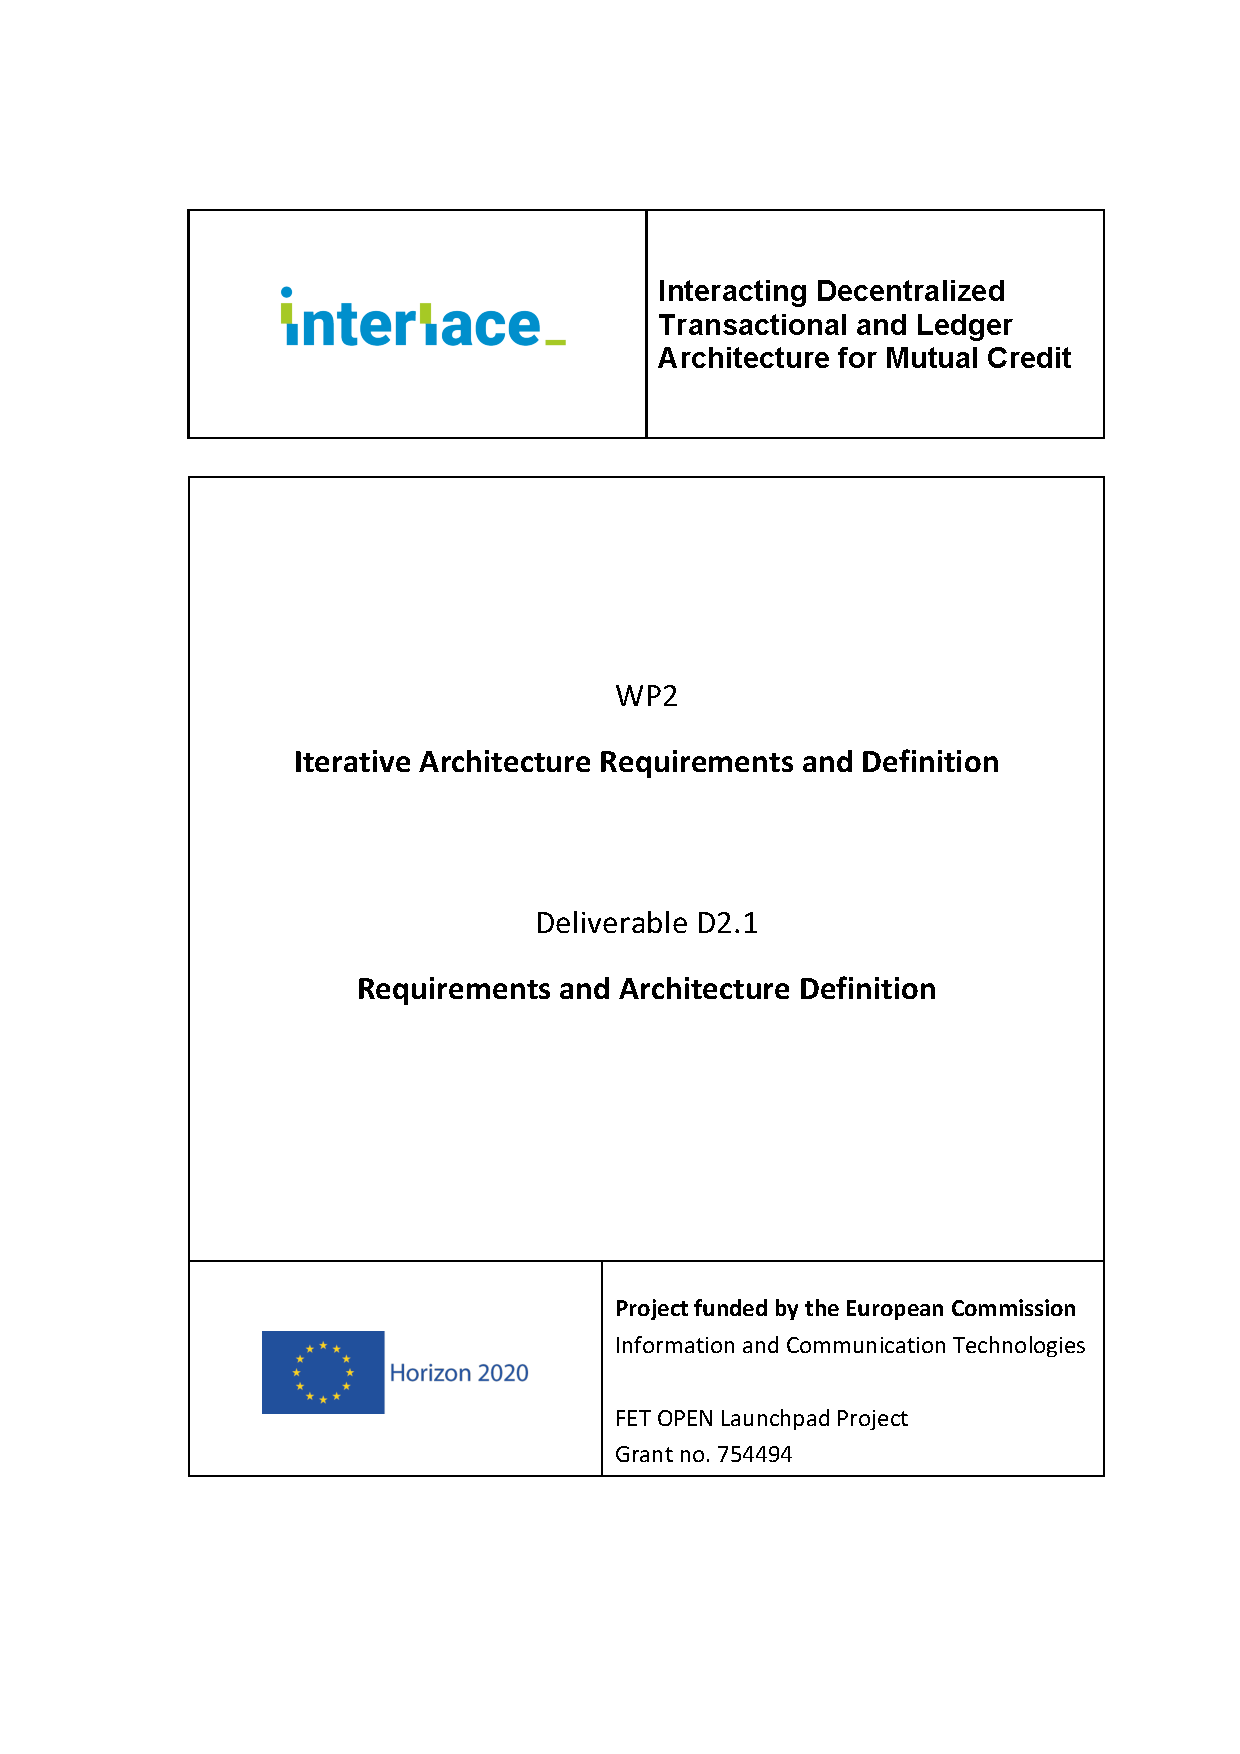
\includepdf[pages=-, scale=1.0]{Misc/Front}

%===================================================
%================== ABSTRACT
%===================================================
\thispagestyle{empty}

\begin{abstract}
\normalsize



\end{abstract}

\newpage

%===================================================
%================== TABLE OF CONTENTS
%===================================================
\tableofcontents

%===================================================
%================== CHAPTERS
%===================================================
\chapter{Introduction}
\label{ch:Introduction}

\vspace{-1cm}
\begin{center}
Paolo Dini and Giuseppe Littera
\end{center}

The INTERLACE project is developing a blockchain-based transactional platform for use by the Sardex mutual credit system. Sardex S.p.A. (SARDEX) has been operating successfully an electronic, B2B, zero-interest mutual credit system on the island of Sardinia since 2009. The Sardex system (also known as Circuito di Credito Commerciale) challenges prevailing notions about the nature of money, and the financial and economic autonomy that a relatively poor region can aspire to, because it enables local economic actors (SMEs in particular) to trade with each other in a trustful and circular fashion with a unique digital trade credit unit. It does this by monetizing the spare capacity of the local economy in the form of mutual, and taxable, credit between participating companies, at zero interest, on a strong basis of trust, solidarity, and local cultural identity \cite{LitteraEtAl2017,DiniMottaSartori2016,SartoriDini2016}. The deeply innovative nature of this system is to distribute to the circuit members the power to create credit money (sardex credits, where 1 credit = 1 Euro), and thereby provide an alternative to credit money creation through bank loans. However, the Sardex transactional platform is currently centralized,\footnote{Cyclos 4: \url{http://www.cyclos.org/products/}.} which challenges the long-term scalability, sustainability, and governance of the system because the governance and management of the circuit are all held by the central credit-clearing entity (SARDEX).

The specification and implementation of the new architecture is based on the Abstract State Interaction Machines (ASIMs), developed and implemented in the platform CoreASIM by the BIOMICS project\footnote{\url{http://biomicsproject.eu/}} \cite{BIOMICSD41,BIOMICSD42,BIOMICSD52} as extensions of B\"orger and St\"ark's \cite{BoergerStaerk2003} Abstract State Machines (ASMs) and of the CoreASM environment.\footnote{\url{http://biomicsproject.eu/news/135-icef}} The ASIMs are based on realizing the BIOMICS mathematical framework for Interaction Machines (IMs) that dynamically and recursively grow and change their components and network topologies to deploy/reabsorb resources in response to interactions and computational needs \cite{NehanivEtAl2015}. Relative to the ASMs, ASIMs are fully asynchronous, concurrent, and communicating, so they can run on different servers and communicate over the network to validate transactions. The ASIM approach is fundamentally important for SARDEX as a company because it guarantees verifiability, validation, and efficient change management (to manage requirements creep as well as new emerging functionalities) through rigorous mathematical formalization of the specification at the level of requirements capture and a rigorous process of iterative refinement down to the level of the code of choice. Any of these levels of abstraction is executable by an interpreter (built into coreASIM), so at each level of the refinement process the current implementation level can be verified against requirements.

The number of new cryptocurrencies is increasing very rapidly,\footnote{As of 28/08/17 there were 865 currencies listed on \url{https://coinmarketcap.com/}, up from 851 a few days earlier.} along with the variations in the technologies that support them. This very volatile technology landscape is causing us to focus first on the new economic and governance model for sardex.net, which will provide the high-level requirements for the new blockchain architecture and will, therefore, enable us to narrow down the number of possible frameworks and technologies to draw from. In the meantime, we have begun the non-trivial task of migrating the current platform functionality towards the new model. The first step in this process has been to begin formalizing the SARDEX business logic as ASM models.

This report is organized as follows. Chapter \ref{ch:archreq} provides a high-level view of the architecture and its documentation following the arc42 method.\footnote{\url{http://arc42.org/}} Chapter \ref{ch:funreq} provides a first collection of functional requirements of the system modelled as ASMs. These reflect the business logic of the \emph{current} system. This model will be instantiated in CoreASIM in order to execute it with a fictitious set of inputs and verify its operation, after which it will be implemented in a language of choice (probably Java).

A second specification and modelling effort will follow, to reflect in the blockchain ``backend'' the new governance and financial/economic model once it has been completed. This second model and its implementation will be reported in the next architecture deliverable (D2.2) at Month 12.












\chapter{High-Level Architectural Requirements and Documentation}
\label{ch:archreq}

\vspace{-1cm}
\begin{center}
Paolo Dini, Eduard Hirsch, Luca Carboni, Massimo Cireddu, Giuseppe Littera, Thomas Heistracher
\end{center}

\section{About INTERLACE}
The objective of INTERLACE is to use the Abstract State Interaction Machines framework (CoreASIM)\footnote{\url{http://biomicsproject.eu/news/135-icef}} open source output of the FP7 FET project BIOMICS to develop a decentralized transactional and ledger architecture demonstrator for B2B mutual credit.

\section{Introduction and Goals}\label{section-introduction-and-goals}
Currently Sardex uses a well running payment platform which offers solid financial transaction facilities in support of B2B trade. Nevertheless, the architecture has been built using a monolithic centralized approach which is not scalable as the system grows in size. In this context, the `system' refers both to the 3500 users in Sardinia as well as the approximately 3000 members across the other 11 circuits in the other Italian regions and the 1500 individual users (members of the Business to Employee, B2E, programme). The aim of the platform redesign is to move to a decentralized and finally to a completely distributed architecture which is able to scale far beyond the capacity of the current implementation. Figure \ref{decentralizedarchitecture} shows the current and the first step in decentralization. It is too early to imagine what form the fully distributed architecture will take, especially since blockchain technology is being innovated and diversifying into different forks at incredible speed. Equally important is the principle according to which the technological architecture should be seen as reflecting and responding to the requirements set by the economic, financial, and governance model. Since this is also evolving, it is more important to develop a tight coupling between a formal but agile specification framework and the corresponding implementation than to have all the architectural answers now.

\begin{figure}[htbp]
\centering
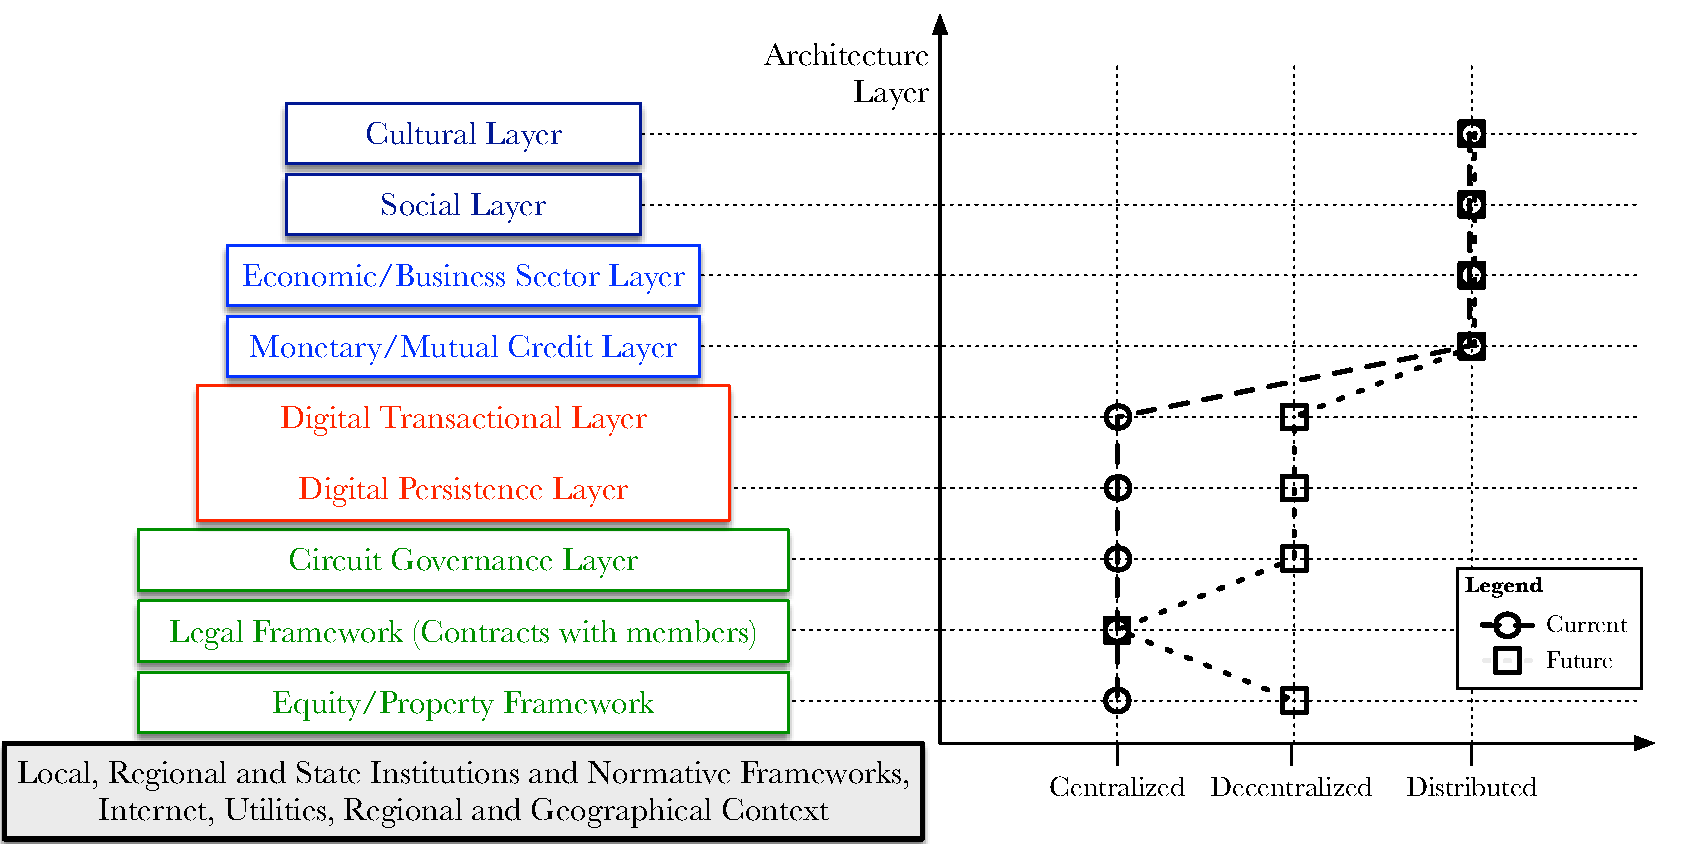
\includegraphics[width=16cm]{Figures/Sardex_Institutional_Structure_V3}
\caption{\small\textbf{Sardex's institutional architecture with current and future decentralization levels}}
\label{decentralizedarchitecture}
\end{figure}

A very powerful, flexible, and formal specification and modelling framework is the ASM method  \cite{BoergerStaerk2003} to develop executable models of the functional requirements. These models will be implemented in the \textbf{coreASIM} framework,\footnote{\url{http://biomicsproject.eu/news/135-icef}} where they can be validated before implementing them in a production environment (e.g.\ in Java).

The INTERLACE proposal describes a blockchain architecture based on the Open Transaction protocol (OTX) \cite{Odom} as an intermediate solution between fully centralized and distributed architectures. OTX involves a pool of Auditor nodes to validate the transactions executed by each Notary node. The initial conception of the INTERLACE architecture was to use only one central Notary, as a first step from the current centralized server towards a more distributed architecture. For the persistence layer we originally examined the Lightweight Cryptocurrency Ledger (LCL) \cite{White2015} as an alternative to the Bitcoin blockchain. The idea of LCL is to store minimal information on the current state of the whole ledger in each block rather than requiring nodes to carry the whole history of block deltas as the Bitcoin blockchain does. This approach achieves continuity with the existing solution while also enabling scalability to multiple circuits (multiple Notaries) under the same mathematical and computational framework.

Rather than replicating the functionality of Cyclos 4 in a decentralized or distributed manner, by implementing the OTX-LCL concepts from scratch, it makes sense to take advantage of the staggering levels of investment currently being made in blockchain technologies by several banking and industry consortia, especially since the best ones are open source, and build on existing frameworks. As of April 2017, just before INTERLACE started, the two most likely candidates for our purposes were IBM's Hyperledger Fabric\footnote{\url{https://hyperledger-fabric.readthedocs.io/en/latest/}}\cite{Cachin2016} and Corda.\footnote{\url{https://www.corda.net/}} Together, they can be described as bringing together the principles of OTX and LCL with the smart contracts of Ethereum.\footnote{\url{https://www.ethereum.org/}} However, an important difference is that these blockchain implementations are �permissioned�, they are not open (�permissionless�) like the Bitcoin or Ethereum blockchains. Although this suits the early decentralised implementation of the INTERLACE blockchain, it opens up governance questions that are currently being examined by Sardex S.p.A. First among these question is the possibility of establishing two separate legal entities:
\begin{packed_item1}
\item Sardex S.p.A. (SARDEX) will maintain its current ownership structure.
\item A new non-profit legal entity, which we can refer to for now as Circuit Coop, or more loosely as sardex.net, may be formed in the near future to begin devolving the ownership of the commons\footnote{The Sardex circuit commons have not been defined yet, but they will constitute a new basis for shared ownership by all the members. An example could be solar panels owned by the coop and providing renewable energy that can only be bought with credits.} to the circuit members.
\end{packed_item1}

From a purely functional point of view, Hyperledger enables a given node to belong to multiple blockchain networks. This is of interest to us because in the governance framework SARDEX is defining at least two units to be stored on the blockchain are envisaged: SRD credits and a new meritocratic reward points system called `Proximity', implemented with tokens that are earned through altruistic behaviour and dubbed `$\pi$'. Corda is interesting because it separates what Hyperledger calls `chaincode', which implements the smart contracts, from the persistence layer. Thus, Corda comes with a `business flow' layer that provides greater flexibility to adapt to the great diversity of actors in the four partially overlapping networks and across different regions or even countries.

The functional requirements addressed in this report cover the core functionalities like credit and debit operations but exclude and intentionally hide implementation details about how transactions are actually processed on the back-end servers. The reason is to enable the ASIMs to communicate directly with the current back-end. After the ASIMs have been verified to execute the current functionalities correctly, the new decentralized/distributed back-end will be developed. Finally, when the new back-end is ready the ASIMs will be changed in order to work with the new logic.

\subsection{Requirements Overview}\label{_requirements_overview}
The requirements have drifted over time due to two causes. First, the technology is changing very quickly, so what we envisaged in terms of technologies at the time of the proposal writing is now obsolete; second, the governance, economic, and financial model of Sardex is \emph{also} evolving, so the high-level requirements themselves have changed relative to a year ago. Therefore, the requirements below will be instantiated in a specific development strategy to be detailed later in this chapter.
\setcounter{table}{0}
\setlength{\tabcolsep}{10pt}
\begin{table}[htbp]
\begin{centering}
\small
{\begin{tabular}{| l | l | }
\hline
\textbf{Req}	& \textbf{Description} \\
\hline
R1 &Needs a transaction layer and a persistence layer\\
\hline
R2 & Both layers must be extensible and scalable to a (global) distributed architecture, \\
&\hspace{0.5cm}but must start decentralized in their initial (local) implementations\\
\hline
R3 &Should be faster than Bitcoin, so a lightweight ledger (fragmented blockchain) approach is preferred	\\
\hline
R4 &Must be able to support intra-trade and inter-trade between multiple circuits. For example, the \\
&\hspace{0.5cm}different circuits could be: \\
&\hspace{1cm}$\bullet$ different Mutual Credit (MC) circuits (Sardex \& Tibex)\\
&\hspace{1cm}$\bullet$ different types of networks (MC circuit and Renewable Energy (RE) network)\\
\hline
R5 &If possible, reuse existing open source solutions and frameworks, within our own customized\\
&\hspace{0.5cm}ASM/ASIM framework \\
\hline
R6 &Chain code (smart contracts code) should be separate from transaction layer for greater speed\\
&\hspace{0.5cm}and efficiency \\
\hline
R7 &Inter-circuit operations must avoid falling under the European PSD2 Directive\\
\hline
R8 &The Sardex blockchain should not have a native token: this is in order to separate unit of account \\
&\hspace{0.5cm}and medium of exchange from the operation of platform (i.e. no mining, as in Bitcoin) and avoid\\
&\hspace{0.5cm}seignorage (as in Ripple/XRP)	\\
\hline
R9 &Smart contracts code can be Turing-complete. The undecidability of Turing-complete languages does\\
&\hspace{0.5cm}not prevent the ability to prove specific properties of specific programs. In the ASM methodology,\\
&\hspace{0.5cm}provability is refined along with the specifications as part of the iterative refinement process,\\
&\hspace{0.5cm}down to the actual code.\\
\hline
R10 &Industry, Academia, NGO, non-profit, Social Movements\\
\hline
R11 &Platform must involve the current regional MC systems and a reward and digital asset system called\\
&\hspace{0.5cm}Proximity and whose unit of account is called $\pi$\\
\hline
R12 &Proximity involves a reward points system whereby $\pi$s are awarded to users on the basis of\\
&\hspace{0.5cm}behaviour that is beneficial for (their local) MC system. Gaining $\pi$s translates into the ability to\\
&\hspace{0.5cm}trade farther away from the user's geographical location. Upon reaching a certain threshold,\\
&\hspace{0.5cm}the user is allowed to trade inter-circuit.  \\
\hline
R13 &The new platform architecture should be closed, i.e.\ `permissioned', both for the regional networks\\
&\hspace{0.5cm}and for Proximity: Open (permissionless) DLT networks like Ripple/XRP could not prevent\\
&\hspace{0.5cm}external actors from speculating on Sardex digital assets like $\pi$. Private (permissioned) DLTs\\
&\hspace{0.5cm}like Chain Core/Ivy (compatible with PSD2) are preferred \\
\hline
R14 &State objects must be immutable: this is important in order to prevent people going back on their\\
&\hspace{0.5cm}commitments, for example the max number of credits they will accept (there are examples of\\
&\hspace{0.5cm}blockchains whose previous blocks have been modified, such as the Ethereum DAO Hack)  \\
\hline
\end{tabular}}
\caption{\small\textbf{Summary of initial high-level requirements}}
\label{ReqTable}
\end{centering}
\end{table}

\subsection{Quality Goals}\label{_quality_goals}

\subsection{Stakeholders and their roles}\label{_stakeholders}

\begin{itemize}
	\item B ... Business
	\item C ... Customer
	\item E ... Employee	
\end{itemize}

\begin{longtable}[]{@{}lll@{}}
\toprule
\begin{minipage}[b]{0.18\columnwidth}\raggedright\strut
Role/Name\strut
\end{minipage} & \begin{minipage}[b]{0.37\columnwidth}\raggedright\strut
Contact\strut
\end{minipage} & \begin{minipage}[b]{0.37\columnwidth}\raggedright\strut
Expectations\strut
\end{minipage}\tabularnewline
\midrule
\endhead
\begin{minipage}[t]{0.18\columnwidth}B2B \end{minipage} &
\begin{minipage}[t]{0.37\columnwidth}Participating Companies \end{minipage} &
\begin{minipage}[t]{0.37\columnwidth}Business to business transactions and interaction\end{minipage}
\tabularnewline
\tabularnewline
\begin{minipage}[t]{0.18\columnwidth}B2E \end{minipage} &
\begin{minipage}[t]{0.37\columnwidth}Employees \end{minipage} &
\begin{minipage}[t]{0.37\columnwidth}Payments of Employees\end{minipage}
\tabularnewline
\tabularnewline
\begin{minipage}[t]{0.18\columnwidth}B2C \end{minipage} &
\begin{minipage}[t]{0.37\columnwidth}Normal Customer \end{minipage} &
\begin{minipage}[t]{0.37\columnwidth}Payments to Participating Companies\end{minipage}
\tabularnewline
\tabularnewline
\begin{minipage}[t]{0.18\columnwidth}Sardex-Admin \end{minipage} &
\begin{minipage}[t]{0.37\columnwidth}Sardex Employee \end{minipage} &
\begin{minipage}[t]{0.37\columnwidth}Configuring and maintaining the infrastructure\end{minipage}
\tabularnewline
\tabularnewline
\begin{minipage}[t]{0.18\columnwidth}Sardex-Manager \end{minipage} &
\begin{minipage}[t]{0.37\columnwidth}Sardex Employee \end{minipage} &
\begin{minipage}[t]{0.37\columnwidth}Running evaluations and managing the cooperation platform \end{minipage}
\tabularnewline


\bottomrule
\end{longtable}

\section{Solution Strategy}\label{section-solution-strategy}
The strategy of how to get from a monolithic working implementation to a decentralized and later a fully distributed ledger application is broken down in several steps, as outlined below.

Since the original ASMs work only in their own scope, it is not possible to create a decentralized or fully distributed environment with them. The solution for the INTERLACE project has been to use a special extension of the ASMs named Abstract Interaction Machines (ASIMs) developed by the BIOMICS project, and a corresponding runtime environment called Interaction Computing Execution Framework (ICEF) \footnote{\url{https://github.com/biomics/icef}}. As explained on the ICEF webpage:
\begin{quote}
\vspace{-0.3cm}
This framework extends the original CoreASM modelling and execution framework to enable the specification and execution of \textbf{distributed and concurrent} ASMs. The ICEF was developed in the STREP project BIOMICS which was financed by the European Comission in FP7 from October 1st, 2012 until March 31st, 2016. ICEF enables asynchronous execution of ASMs. It uses and enhances the CoreASM execution engine to support communicating and interacting ASMs: CoreASIMs. Further, ICEF replaces ASM with BSL which offers additional language primitives specifically designed to define the beahviour of biochemical systems. This code introduces a restful API to control the BIOMICS wrapper (brapper) which can host several CoreASIM instances and enables networked CoreASIM. It also introduces a manager which orchestrates several ASIMs to allow the execution of interaction computing simulations.
\end{quote}

Although the additional language primitives offered by ICEF might not be needed, the coreASIM implementation will be crucial for realizing the INTERLACE strategy.

\subsection{Strategy Steps}\label{subsection-strategy-steps}

\begin{enumerate}
	\item Define the functional requirements of the business logic using the ASMs formal description language (this report).
	\item Translate the formal description to a working demo environment using ICEF/coreASIM.
	\item Connect the business logic modelled with ASMs and implemented in coreASIM to the real world. That means use the interaction capabilities of the framework to connect it to the existing legacy application used by SARDEX, Cyclos 4. This existing working architecture is summarized at a high level in Figure \ref{cyclosarchitecture}.
	\item Test if the application and the translation to coreASIM work.
	\item Translate the coreASIM implementation to a real-world application by creating e.g.\ a JAVA. application.
	\item Develop a verification strategy and validate the implemented real-world application through component testing.
	\item Select appropriate blockchain technologies for the next-generation infrastructure.
	\item Develop ASIM specifications that model the distributed environment.
	\item Adapt ASIM interfaces.
	\item Adapt the real-world version of the application to the new infrastructure.
	\item Implement the new back-end logic using Open Source frameworks.
	\item Test/Validate with real users the new application against the new back-end.
\end{enumerate}


\begin{figure}[htbp]
\centering
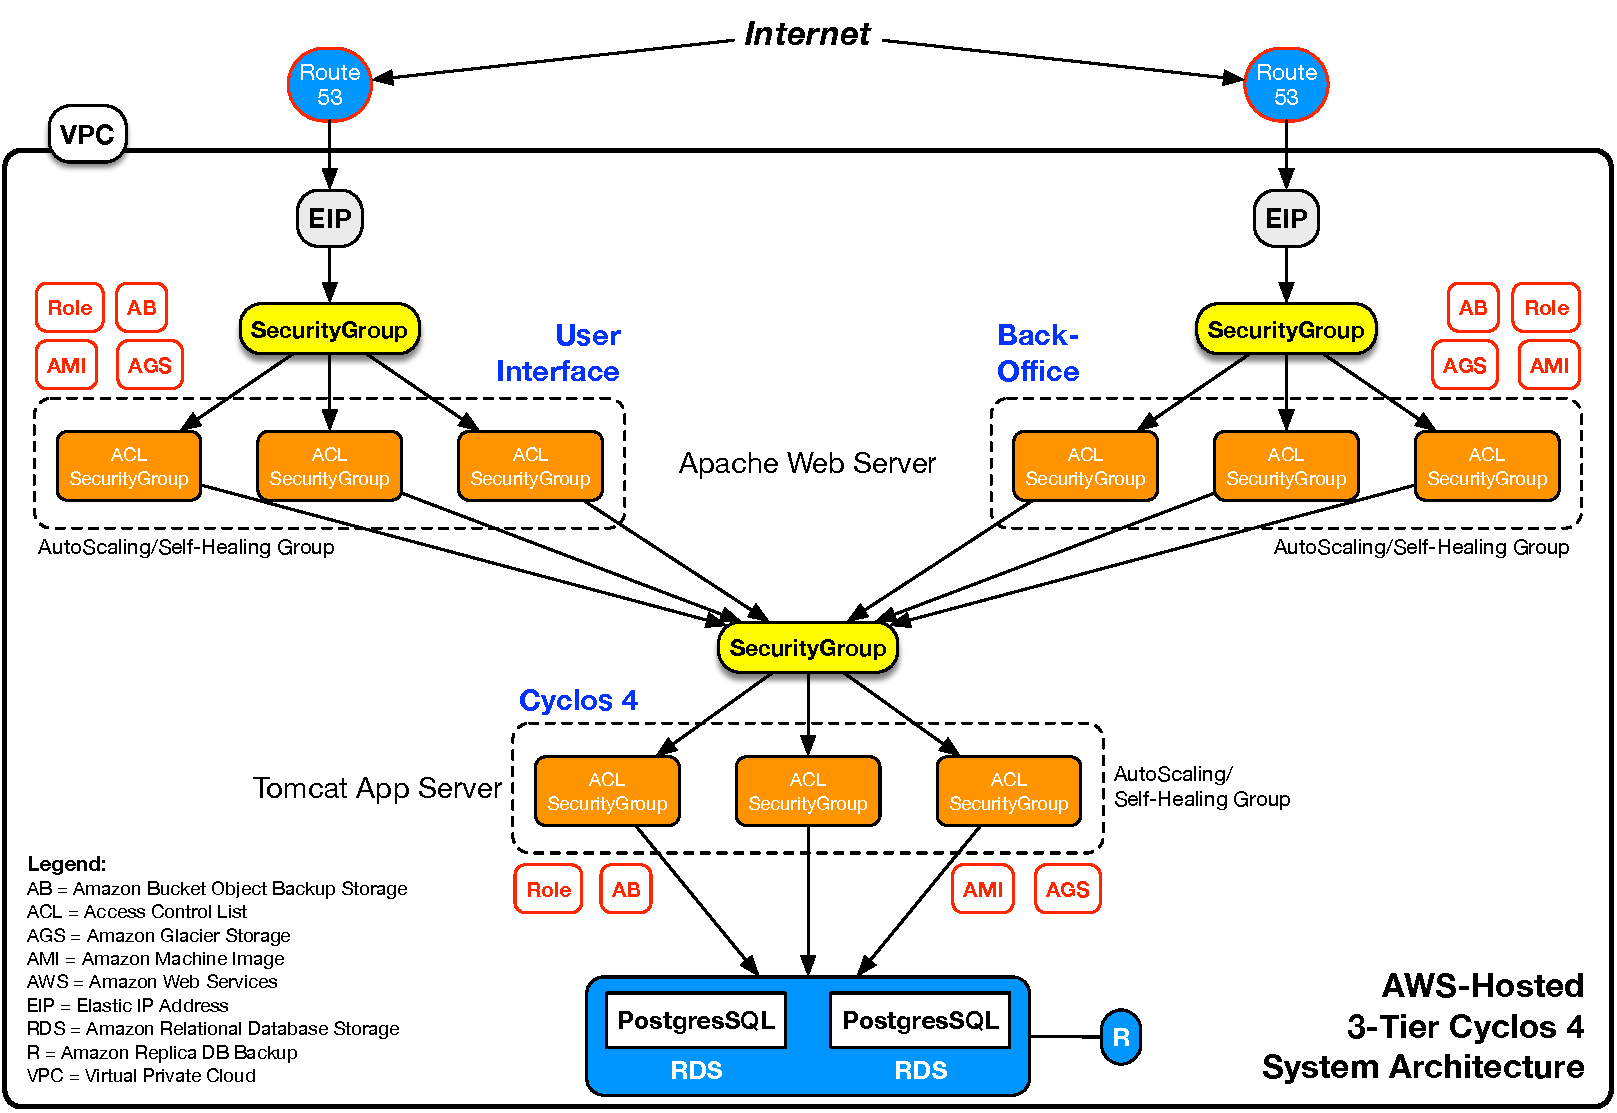
\includegraphics[width=17.5cm]{Figures/3-Tier_Cyclos_Architecture}
\caption{\small\textbf{Existing 3-tier Cyclos 4 architecture used by SARDEX, based on Amazon Web Services}}
\label{cyclosarchitecture}
\end{figure}




%\section{Architecture
%Constraints}\label{section-architecture-constraints}

%\section{System Scope and
%Context}\label{section-system-scope-and-context}

%\subsection{Business Context}\label{_business_context}

%\textbf{\textless{}Diagram or Table\textgreater{}}

%\textbf{\textless{}optionally: Explanation of external domain
%interfaces\textgreater{}}

%\subsection{Technical Context}\label{_technical_context}

%\textbf{\textless{}Diagram or Table\textgreater{}}

%\textbf{\textless{}optionally: Explanation of technical
%interfaces\textgreater{}}

%\textbf{\textless{}Mapping Input/Output to Channels\textgreater{}}

%\section{Solution Strategy}\label{section-solution-strategy}

%\section{Building Block View}\label{section-building-block-view}

%\subsection{Whitebox Overall System}\label{_whitebox_overall_system}

%\emph{\textbf{\textless{}Overview Diagram\textgreater{}}}

%\begin{description}
%\item[Motivation]
%\emph{\textless{}text explanation\textgreater{}}
%\item[Contained Building Blocks]
%\emph{\textless{}Description of contained building block (black
%boxes)\textgreater{}}
%\item[Important Interfaces]
%\emph{\textless{}Description of important interfaces\textgreater{}}
%\end{description}

%\subsubsection{\textless{}Name black box
%1\textgreater{}}\label{__name_black_box_1}

%\emph{\textless{}Purpose/Responsibility\textgreater{}}

%\emph{\textless{}Interface(s)\textgreater{}}

%\emph{\textless{}(Optional) Quality/Performance
%Characteristics\textgreater{}}

%\emph{\textless{}(Optional) Directory/File Location\textgreater{}}

%\emph{\textless{}(Optional) Fulfilled Requirements\textgreater{}}

%\emph{\textless{}(optional) Open Issues/Problems/Risks\textgreater{}}

%\subsubsection{\textless{}Name black box
%2\textgreater{}}\label{__name_black_box_2}

%\emph{\textless{}black box template\textgreater{}}

%\subsubsection{\textless{}Name black box
%n\textgreater{}}\label{__name_black_box_n}

%\emph{\textless{}black box template\textgreater{}}

%\subsubsection{\textless{}Name interface
%1\textgreater{}}\label{__name_interface_1}

%\ldots{}

%\subsubsection{\textless{}Name interface
%m\textgreater{}}\label{__name_interface_m}

%\subsection{Level 2}\label{_level_2}

%\subsubsection{\texorpdfstring{White Box \emph{\textless{}building block
%1\textgreater{}}}{White Box \textless{}building block 1\textgreater{}}}\label{_white_box_emphasis_building_block_1_emphasis}

%\emph{\textless{}white box template\textgreater{}}

%\subsubsection{\texorpdfstring{White Box \emph{\textless{}building block
%2\textgreater{}}}{White Box \textless{}building block 2\textgreater{}}}\label{_white_box_emphasis_building_block_2_emphasis}

%\emph{\textless{}white box template\textgreater{}}

%\ldots{}

%\subsubsection{\texorpdfstring{White Box \emph{\textless{}building block
%m\textgreater{}}}{White Box \textless{}building block m\textgreater{}}}\label{_white_box_emphasis_building_block_m_emphasis}

%\emph{\textless{}white box template\textgreater{}}

%\subsection{Level 3}\label{_level_3}

%\subsubsection{White Box \textless{}\_building block
%x.1\_\textgreater{}}\label{_white_box_building_block_x_1}

%\emph{\textless{}white box template\textgreater{}}

%\subsubsection{White Box \textless{}\_building block
%x.2\_\textgreater{}}\label{_white_box_building_block_x_2}

%\emph{\textless{}white box template\textgreater{}}

%\subsubsection{White Box \textless{}\_building block
%y.1\_\textgreater{}}\label{_white_box_building_block_y_1}

%\emph{\textless{}white box template\textgreater{}}

%\section{Runtime View}\label{section-runtime-view}

%\subsection{\textless{}Runtime Scenario
%1\textgreater{}}\label{__runtime_scenario_1}

%\begin{itemize}
%\item
%  \emph{\textless{}insert runtime diagram or textual description of the
%  scenario\textgreater{}}
%\item
%  \emph{\textless{}insert description of the notable aspects of the
%  interactions between the building block instances depicted in this
%  diagram.\textgreater{}}
%\end{itemize}

%\subsection{\textless{}Runtime Scenario
%2\textgreater{}}\label{__runtime_scenario_2}

%\subsection{\ldots{}}\label{_}

%\subsection{\textless{}Runtime Scenario
%n\textgreater{}}\label{__runtime_scenario_n}

%\section{Deployment View}\label{section-deployment-view}

%\subsection{Infrastructure Level 1}\label{_infrastructure_level_1}

%\emph{\textbf{\textless{}Overview Diagram\textgreater{}}}

%\begin{description}
%\item[Motivation]
%\emph{\textless{}explanation in text form\textgreater{}}
%\item[Quality and/or Performance Features]
%\emph{\textless{}explanation in text form\textgreater{}}
%\item[Mapping of Building Blocks to Infrastructure]
%\emph{\textless{}description of the mapping\textgreater{}}
%\end{description}

%\subsection{Infrastructure Level 2}\label{_infrastructure_level_2}

%\subsubsection{\texorpdfstring{\emph{\textless{}Infrastructure Element
%1\textgreater{}}}{\textless{}Infrastructure Element 1\textgreater{}}}\label{__emphasis_infrastructure_element_1_emphasis}

%\emph{\textless{}diagram + explanation\textgreater{}}

%\subsubsection{\texorpdfstring{\emph{\textless{}Infrastructure Element
%2\textgreater{}}}{\textless{}Infrastructure Element 2\textgreater{}}}\label{__emphasis_infrastructure_element_2_emphasis}

%\emph{\textless{}diagram + explanation\textgreater{}}

%\ldots{}

%\subsubsection{\texorpdfstring{\emph{\textless{}Infrastructure Element
%n\textgreater{}}}{\textless{}Infrastructure Element n\textgreater{}}}\label{__emphasis_infrastructure_element_n_emphasis}

%\emph{\textless{}diagram + explanation\textgreater{}}

%\section{Cross-cutting Concepts}\label{section-concepts}

%\subsection{\texorpdfstring{\emph{\textless{}Concept
%1\textgreater{}}}{\textless{}Concept 1\textgreater{}}}\label{__emphasis_concept_1_emphasis}

%\emph{\textless{}explanation\textgreater{}}

%\subsection{\texorpdfstring{\emph{\textless{}Concept
%2\textgreater{}}}{\textless{}Concept 2\textgreater{}}}\label{__emphasis_concept_2_emphasis}

%\emph{\textless{}explanation\textgreater{}}

%\ldots{}

%\subsection{\texorpdfstring{\emph{\textless{}Concept
%n\textgreater{}}}{\textless{}Concept n\textgreater{}}}\label{__emphasis_concept_n_emphasis}

%\emph{\textless{}explanation\textgreater{}}

%\section{Design Decisions}\label{section-design-decisions}

%\section{Quality Requirements}\label{section-quality-scenarios}

%\subsection{Quality Tree}\label{_quality_tree}

%\subsection{Quality Scenarios}\label{_quality_scenarios}

\section{Risks and Technical Debts}\label{section-technical-risks}

\section{Glossary}\label{section-glossary}

\begin{longtable}[]{@{}ll@{}}
\toprule
\begin{minipage}[b]{0.47\columnwidth}\raggedright\strut
Term\strut
\end{minipage} & \begin{minipage}[b]{0.47\columnwidth}\raggedright\strut
Definition\strut
\end{minipage}\tabularnewline
\midrule
\endhead
\begin{minipage}[t]{0.47\columnwidth}\raggedright\strut
\textless{}Term-1\textgreater{}\strut
\end{minipage} & \begin{minipage}[t]{0.47\columnwidth}\raggedright\strut
\textless{}definition-1\textgreater{}\strut
\end{minipage}\tabularnewline
\begin{minipage}[t]{0.47\columnwidth}\raggedright\strut
\textless{}Term-2\textgreater{}\strut
\end{minipage} & \begin{minipage}[t]{0.47\columnwidth}\raggedright\strut
\textless{}definition-2\textgreater{}\strut
\end{minipage}\tabularnewline
\bottomrule
\end{longtable}

\chapter{Functional Requirements and Business Logic}
\label{ch:funreq}


\vspace{-1cm}
\begin{center}
Egon B\"orger, Luca Carboni, Massimeddu Cireddu, Paolo Dini, Eduard Hirsch, Giuseppe Littera
\end{center}


We specify the core payment and related history operations of the Sardex system. We do this at the functional requirements  level of abstraction and in a component-based manner so that the resulting model can serve as abstract description of the current implementation but also as starting point for a new, blockchain-based implementation. Sect.~\ref{sect:paymtops} models  two basic payment operations, Sect.~\ref{sect:accHistory} account history and balance operations, Sect.~\ref{sect:userops} user operations. Permission features and onboarding operations will be modelled in the near future and reported on in the next deliverable (D2.2).


\section{Core Payment Operations}
\label{sect:paymtops}

In this section we describe the interaction of the Sardex system (also called simply Sardex)  with users. We consider here only B2B operations, leaving the consideration of operations between a $Company$ and either $Employee$s or $Consumer$s for a later phase. Sect.~\ref{signaturepaymtop} explains the basic data types,  Sect.~\ref{sec:creditop} the credit and  Sect.~\ref{sec:debitop} the debit operation.

\subsection{Signature elements of B2B Operations}
\label{signaturepaymtop}
The actors of B2B operations are companies (elements of the set $Company$) which interact with the Sardex system on a request/response basis using various communication devices from whose technical details we abstract here. Therefore it comes natural to describe the interaction of companies with the Sardex system by $\ASM{Send}$ and $\ASM{Receive}$ actions of communicating Abstract State Machines (ASMs), the basic concept underlying Abstract State Interaction Machines (ASIMs)\footnote{ASIMs are communicating ASMs which are equipped with a general scheduling mechanism and an interaction structure to distinguish between horizontal and hierarchical interaction. These features have been defined to satisfy the requirements of Interaction Computing formulated in Deliverable 5.1 of the BIOMICS project  \cite{BIOMICSD51}; these requirements have been shown to be satisfied by ASIMs (see Ch.\ 2 of Deliverable D5.2 \cite{BIOMICSD52}). For further details (in particular on the definition of the communication network structure, using channels and a routing component, and a resource manager by specialized communicating ASMs) and the implementation see \url{https://github.com/biomics/icef}.}, one for each participating company and one for Sardex.\footnote{Observe that in a distributed version of the Sardex system different instances of the system are run by different agents which all execute the same ASM program (or a program that has been obtained by adapting the basic program appropriately for a particular instance). Cyclos today is loosely coupled in the sense that one can have multiple applications running on multiple machines that share consistency with third-party utilities.} We concentrate our attention in this section on modelling the actions the Sardex system performs when triggered by requests sent to it by any company of the circuit (which are treated in Sec.~\ref{sect:userops}).

We keep the communication mechanism abstract. $\ASM{Send}(msg,\TO :a)$ denotes the operation of sending the $msg$ to agent $a$. 
$Received(msg,\FROM :s)$ is a predicate which is true when the message $msg$ from the sender $s$ is in the $mailbox$ of the receiver. $\ASM{Consume}(msg)$ denotes the operation of deleting the $msg$ from the $mailbox$ once it has been processed. Thus,
the �from/to:� notation does not describe a function; it is used for the convenience of reading a rule where it only makes a parameter explicit that is used in the rule and anyway assumed to be part of the message in question.

We usually assume  each $msg \in Message$ to contain besides its $payload(msg)$ also the information about its $sender(msg)$ and $receiver(msg)$. Thus the parameter $\FROM :c$ in $Received(msg, \FROM :c)$ indicates that $sender(msg)=c$. Similarly, $\TO :c$ in $\ASM{Send}(msg, \TO :c)$ denotes that $receiver(msg) = c$.

The core payment operations are sent to Sardex by companies $c \in SardexNet$ which are members of the net.\footnote{We use for the datatypes evocative names which suggest their intended interpretation.} Each such company may have a number of $acc$ounts\footnote{A company can have at most an account for each account type.} which we represent as elements of a set $Account(c)$. Each $acc$ount has a well-defined $owner(acc) \in SardexNet$ and is of some type $accountType(acc)$ out of the set $AccountType$ of possible account types:

\begin{asm}
AccountType=\{credit, domu, fee\} \\
Account = \bigcup_{c \in SardexNet} Account(c)
\end{asm}
Therefore we name such accounts $creditAccount(c)$, $domuAccount(c)$, $feeAccount(c)$ (names which are defined if $c$ has the corresponding accounts). 

There are two principal transfer operations, called Credit and Debit operation specified in Sec.~\ref{sec:creditop} and Sec.~\ref{sec:debitop}.

\subsection{Sardex Behaviour for Credit Operations}
\label{sec:creditop}

A Credit operation is also called a push transfer. Its goal is to transfer an $amount$ via a specific $channel$ from one account to another. Sardex uses a $TransferType$ concept which allows one to impose on the transfer operations certain conditions, including priorities. The parameters of a transfer type $tt$ which are relevant for the Sardex business logic are the following:\footnote{The implementation in Cyclos has more parameters we do not consider here.}
\begin{itemize}
	\item the $operation \in \{credit, debit\}$,
	\item the $channel \in \{phone,website,pos\}$\footnote{$pos$ abbreviates point of sale.} through which the interaction between the user and Sardex takes place,
	\item the account type of the two involved accounts $from,to \in Account$,
	\item the groups of the two members involved: $fromMbrGroup,toMbrGroup \in Group$,
	\item conditions on the to-be-transferred $amount$, 
	\item conditions on so-called custom fields.
\end{itemize}

$CustField$ is a set of typed variables, with or without parameters, in ASM terminology a set of 0-ary or $n$-ary functions (with $n>0$) whose values are of an indicated type. They serve to encode customer information on the reason of a transfer, e.g. the number and date of the bill to be paid. For each transfer type $tt$ its $custFields(tt)$ (if there are any) are of two kinds, compulsory or optional. Optional fields do not affect the $custFieldCond$ition of a transfer type. For a $transfer$ to $Match$ a transfer type $tt$ means in particular that its $custFieldCond(tt,custFields(transfer))$ evaluates to true, where $custFields(transfer)$ denotes the values of the custom fields in the $transfer$. As a consequence if a transfer type $tt$ comes without or only with optional custom fields, then the $custFieldCond$ with $tt$ as first argument is empty, i.e. simply true.

We retrieve for each parameter the corresponding information from a transfer type $tt$ by an appropriate function:

\begin{asm}
name\colon TransferType \rightarrow Identifier \\
oper\colon TransferType \rightarrow Operation\\
chan\colon TransferType \rightarrow Channel \\
sourceType,destType\colon TransferType \rightarrow Formula 
       \mbox{ // expressions for conditions}\\
fromMemberGroup,toMemberGroup \colon TransferType \rightarrow Group \\
amountCond,custFieldCond\colon TransferType \rightarrow Formula\\
\WHERE \+
    Operation = \{credit,debit\} \\
    Channel = \{phone, website,pos\}
\end{asm} 

One can imagine $TransferType$ as a table where each row is named and contains the parameters of the represented $tt$. The $TransferType$ data type is defined in such a way as to guarantee the following property: 
\begin{quote} 
	{\bf Transfer Type Welldefinedness}. For each transfer $operation \in \{credit,debit\}$, each pair of accounts $acc,acc'$ and each $channel$ there is at most one $tt \in TransferType$, i.e. at most one $tt$ which satisfies
	\begin{itemize}
		\item $oper(tt) = operation$,
		\item $chan(tt)=channel$,
		\item $sourceType(tt)=accountType(acc)$,
		\item $destType(tt)=accountType(acc')$.
	\end{itemize} 
We denote this unique $tt$ as the value of the function $tt(operation,acc,acc',channel)$.\footnote{Following common notation we use the same name $tt$ for elements of $TransferTable$ and for the function $tt(params)$; it will always be clear from the context which one is meant.}
\end{quote}


Both payment operations Credit and Debit are instances of a request/response pattern with two phases, a first phase whose action is called Preview -- where only the permission for the transfer is checked (using a $transferTypeCheck$ function) but not the requested amount -- and  a second phase whose action is called Perform where also the amount is checked (using a $balanceCheck$ function). On the user side both actions are treated as stateless, on the Sardex system side only the Preview action is stateless. Here we make the -- for the user stateless -- two-phase interaction explicit by using two  types of user requests, say $CreditPreviewReq$ and $CreditPerformReq$, with corresponding Sardex rules $\ASM{CreditPreviewReq}$ and $\ASM{CreditPerformReq}$ to react to such requests. The user first sends a $CreditPreviewReq$uest and upon the positive system response the corresponding $CreditPerformReq$uest. Sardex can execute at any moment any of its $\ASM{CreditTransferReq}$ rules whose execution depends only on the parameters with which they are called. But for one successful credit request instance the two rules can be executed only in the indicated order, due to the intrinsic sequentiality of the two steps for the request.

{\bf Remark}. In the $\ASM{CreditTransferReq}$ model we assume that its access to the two accounts $from, to$ is exclusive. This assumption plays the role of a constraint for the implementation and thus is an essential part of the specification. We do not model the corresponding synchronization mechanism (which guarantees the assumption) because its functionality is clear and it is well-known how to program it. 

\begin{asm}
\ASM{CreditTransferReq}((channel,from, to, amount),mbr)=\+
   \ASM{CreditPreviewReq}((channel,from,to,amount),mbr)  \\
   \ASM{CreditPerformReq}((channel,from,to,amount),mbr) 
\end{asm}


We define the two core functions $transferTypeCheck$ and $balanceCheck$ of $\ASM{CreditTransferReq}$ abstractly, to satisfy a modular design approach, as yielding either a positive answer -- for $transferTypeCheck$ (in this case by the Transfer Type Welldefinedness property stated above) the matching type $tt$ and for $balanceCheck$  the answer OK -- or some information on the reason why the check did not succeed. Since there may be several reasons for a failure, in case of failure the value of the two functions is a set of detected failure reasons, say elements of $TransferTypeError$ resp. $BalanceViolation$.  Out of this set an $ErrMsg$ can be constructed to provide the user with some information why the check did not succeed, tailoring the format and payload of error messages.  Below we illustrate this modular approach to exception handling by some characteristic examples.


\begin{asm}
\ASM{CreditPreviewReq}((channel,from,to,amount,custFlds),mbr)  =\+
  \IF  Received(CreditPreviewReq
        (credit,channel,from,to,amount,custFlds),\FROM :mbr) \THEN \+  
    \LET transfer = (credit,channel,from,to,amount,custFlds) \\
    \LET ttRes = transferTypeCheck(transfer)  \+
      \IF ttRes \not \in TransferType \THEN \+   
         \ASM{Send}(ErrMsg(NotPermitted(transfer,ttRes)),\TO :mbr)\-
      \ELSE~  \ASM{Send}(YouMayProceedWith(transfer),\TO :mbr)\-
    \ASM{Consume}(CreditPreviewReq
        (credit,channel,from,to,amount,custFlds),\FROM :mbr) \dec\-
\WHERE \+
  transferTypeCheck(transfer) \in \+
           \left\{\begin{array}{ll}
           \{tt\} & \IF  tt \in TransferType \AND    
           Match(tt,transfer)\\
           PowerSet(TransferTypeError) & \ELSE 
           \end{array}\right .\-
Match(tt,transfer) \IF \+
          oper(tt)=credit \AND chan(tt)=channel \AND \\
          owner(from) \in fromMemberGroup(tt) \AND 
              owner(to) \in toMemberGroup(tt)  \AND \\
          sourceType(tt)=accountType(from) \AND destType(tt)=accountType(to) \AND \\
              custFieldCond(tt,custFlds)=true\dec\-
\end{asm}


The $Match$ predicate is extended in Sec.~\ref{sec:debitop} for the first transfer parameter $debit$ (instead of $credit$).\footnote{This is the reason why the definition here considers only the $\IF$ case instead of stating $\IFF$.} The set of possible $TransferTypeError$s can be defined for the various cases of interest where
the $Match(tt,transfer)$ condition is violated for whatever $tt \in TransferType$.


Since Sardex when responding to a $CreditPreviewReq$uest does not record the data (due to the requirement of the stateless Preview response character), when elaborating a $CreditPerformReq$uest the system in a first step must redo the $transferTypeCheck$. In the case of a positive check result, as part of the $transaction$ which is added to the $Ledger$, besides the $transfer$ parameters also the computed transfer type is recorded together with the transfer date (which is computed by the system as value of a location, say $today$, when the credit request is performed). The function $transaction$ denotes the final transaction corresponding to the given $transfer$, its date and transfer type. 

To formulate error conditions for the $balanceCheck$ we need a function $availBalance(acc)$ which yields the amount of money that is currently available in the $acc$ to be spent. It is defined together with the related current balance function $balance(acc)$ in Sect.~\ref{sect:accHistory}. $Receivable(amount,acc)$ checks whether the destination of the transfer by receiving the $amount$ would exceed its upper Sardex limit $upperLimit(acc)$.


\begin{asm}
\ASM{CreditPerformReq}((channel,from,to,amount,custFlds),mbr)=\+
\IF Received
   (CreditPerformReq(credit,channel,from,to,amount,custFlds),\FROM :mbr) \THEN \+  \LET transfer=(credit,channel,from,to,amount,custFlds) \\
    \LET ttRes=transferTypeCheck(transfer)  \+
      \IF ttRes \not \in TransferType \THEN \+ \ASM{Send}(ErrMsg(NotPermitted(transfer,ttRes)),\TO :mbr)\-
       \ELSE~ 
       \LET bal = balanceCheck(from, to, amount) \+
              \IF bal = OK \+
                 \THEN \+
                      \ASM{Append}(transaction(transfer,ttRes,today),Ledger)\\
                      \ASM{Send}(Confirmed(transfer),\TO :mbr)\-
                \ELSE ~ \ASM{Send}(ErrMsg(transfer,bal),\TO :mbr)\dec\dec\-
    \ASM{Consume}(CreditPerformReq(channel,from,to,amount,custFlds),\FROM : mbr) \dec\-
\WHERE \+
balanceCheck(from, to, amount) \in \{OK\} 
                  \cup Powerset(BalanceViolation)\\
balanceCheck(from, to, amount) = OK \IFF 
         amountCond(ttRes)(amount) =true \AND \+
         availBalance(from) \geq amount  \AND Receivable(amount,to)\-
ViolatesAmountCond(amount) \IF  amountCond(ttRes)(amount) = false \\
ViolatesLowerLimit(from,amount) \IF availBalance(from) < amount \\
ViolatesUpperLimit(to,amount) \IF ~\NOT Receivable(amount,to) \\
 Receivable(amt,acc) \mbox{ iff } balance(acc) + amt \leq upperLimit(acc)
\end{asm}



\subsection{Sardex Behaviour for Debit Operations}
\label{sec:debitop}

In the Sardex business logic also a Debit transfer can be performed but only between accounts of type $credit$ (neither $domu$ nor $fee$). Since any Sardex member $c \in SardexNet$ can be $owner$ of at most one account of type $credit$, Debit transfers are formulated as being performed among members $creditor,debitor$. Sardex accepts a $DebitPreviewReq$uest and a  $DebitPerformReq$uest from a $creditor$, using two corresponding rules $\ASM{DebitPreviewReq}$ and $\ASM{DebitPerformReq}$ Sardex uses to interact with the $creditor$.  $DebitPerformReq$uests are executed using a request/response interaction between the system and the $debitor$. The $debitor$ has to allow the transfer by acknowledging a $ConfirmationReq$uest Sardex sends out; only when the debit transfer has been permitted by an acknowledgement from the $debitor$ will Sardex execute the transfer using a third rule called $\ASM{DebitAckExec}$ution. 

Sardex can execute at any moment any of these rules whose execution depends only on the parameters with which they are called. But for one successful debit $request$ instance the three rules can be executed only in the indicated order, due to the intrinsic sequentiality of the three steps for the $request$.

{\bf Remark}. As for $\ASM{CreditTransferReq}$ also in the $\ASM{DebitTransferReq}$ model we assume that the access to the two accounts $from, to$ is exclusive (synchronization constraint). 


\begin{asm}
\ASM{DebitTransferReq}=\+
   \ASM{DebitPreviewReq} \\
   \ASM{DebitPerformReq} \\
   \ASM{DebitAckExec}
\end{asm}


Both rules $\ASM{DebitPreviewReq}$ and $\ASM{DebitPerformReq}$ in their first step make a $transferTypeCheck$ for the account of type $credit$ of the $debitor$, defined by extending the $Match$ predicate for $debit$ transfer operations. This extension works for B2B operations; it also works for B2E but not for E2B or E2E. In other words $Employee$s are not allowed to request (i.e. appear as first argument of) a Debit transfer.

\begin{asm}
\ASM{DebitPreviewReq}((debitor,channel,amount,custFlds),creditor)=\+
  \IF Received(DebitPreviewReq(debitor,channel,amount,custFlds),
                   \FROM :creditor) \THEN \+  
     \LET from=creditAccount(creditor), to=creditAccount(debitor)\\
     \LET transfer=(debit,channel,from,to,amount,custFlds)\\  
     \LET ttRes=transferTypeCheck(transfer) \+
        \IF ttRes \not \in TransferType \THEN \+    \ASM{Send}(ErrMsg(NotPermitted(transfer,ttRes)),\TO :creditor)\-
       \ELSE~  \ASM{Send}(YouMayProceedWith(transfer),\TO :creditor)\dec\-
   \ASM{Consume}(DebitPreviewReq(debitor,channel,amount,custFlds),
                   \FROM :creditor) \-
\WHERE \+
   Match(tt,transfer) \IF \+
      oper(tt)=debit \AND chan(tt)=channel \AND \\
          owner(from) \in fromMemberGroup(tt) \AND 
              owner(to) \in toMemberGroup(tt)  \AND \\
          sourceType(tt)=accountType(from) \AND destType(tt)=accountType(to) \AND \\
              custFieldCond(tt,custFlds)=true
\end{asm}


If the $transferTypeCheck$ in a $ \ASM{DebitPerformReq}$uest succeeds, a two-phase request/response interaction is started, this time with the system as requestor with the $debitor$ to respond. More precisely, upon receiving the $DebitPerformReq$uest from the $creditor$, the system after a successful  $transferTypeCheck$ executes a $balanceCheck$, for which we can use the same abstract function as for Credit operations but with interchanged source/destination parameters; in other words, the system checks whether from the $creditAccount(debitor)$ a corresponding Credit operation can be performed. If this check succeeds the system inserts the transaction without further ado if the amount is small (less than 100). Otherwise it creates a $OneTimePassword$ $otp$, records its birthtime (the beginning of its lifetime), records the $otp$ with the transaction (including the computed transfer type) as pending transaction and sends the $otp$  with an agreement request to the $debitor$. It then waits for a confirmation.


\begin{asm}
\ASM{DebitPerformReq}((debitor,channel,amount,custFlds),creditor)=\+
\IF  Received(DebitPerformReq(debitor,channel,amount,custFlds),
                 \FROM :creditor) \THEN \+     
  \LET from=creditAccount(creditor), to=creditAccount(debitor)\\
  \LET transfer=(debit,channel,from,to,amount,custFlds) \\
  \LET ttRes=transferTypeCheck(transfer) \+
        \IF ttRes \not \in TransferType \THEN \+    \ASM{Send}(ErrMsg(NotPermitted(transfer,ttRes)),\TO :creditor)\-
       \ELSE~  \LET bal = balanceCheck(to, from, amount)  
                \mbox{ // check balance}\+
       \IF bal \not =ok \THEN ~ \ASM{Send}(ErrMsg(transfer,bal),\TO :creditor)   \ELSE \+
         \IF Small(amount) \+
              \THEN \+ 
                   \ASM{Append}(transaction(transfer,ttRes,today),Ledger) \\
                   \ASM{Send}(Confirmed(transfer,ttRes,today),\TO :creditor)\\
                   \ASM{Send}(Confirmed(transfer,ttRes,today),\TO : debitor)\-
              \ELSE ~ \LET otp= \NEW(OneTimePassword)\+
                  birthTime(otp):=now \mbox{ // current system time}\\
                  \ASM{Insert}((otp,transaction(transfer,ttRes)),PendingTransaction)\\ 
                   status((otp,transaction(transfer,ttRes))):=pending \\
                   \ASM{Send}(ConfirmationReq
                    (amount,creditor,otp),\TO :debitor)\dec\dec\dec\dec\-
   \ASM{Consume}(DebitPerformReq(debitor,channel,amount,custFlds),
                 \FROM :creditor)
\end{asm}
             
When the $otp$ is acknowledged (i.e. resent) by the $debitor$ 
within the $lifetimeForOTPs$ forseen for one time passwords, the system updates the transaction status from $pending$ to $performed$ and 
$\ASM{Append}$s the transaction to the $Ledger$ with the current date $today$. When the system is waiting for an $otp$ confirmation the $debitor$ is expected to send, this member may instead try to make another Credit transfer. In this case it could be that only one, Credit or Debit, is still possible due to the $debitor$'s account balance. For this reason, when the pending transaction is confirmed, the $balanceCheck$  (but not any more the $transferTypeCheck$) is performed once more and only when it succeeds is the transaction put into the $Ledger$. The one time password is deleted to avoid a later application of the rule which has to be applied in case of an $Expired(otp)$. 
              
 \begin{asm}  
 \ASM{DebitAckExec} =\+           
\IF Received
     (DebitAckMsg(amount,creditor,otp),\FROM :debitor) and \NOT Expired(otp) \THEN \+ 
  \IF ~ \THEREISNO t \in PendingTransaction \WITH fst(t)=otp\footnote{$fst$ denotes the first element of a sequence, here of a pair $(otp,t)$ of an $otp$ and the corresponding pending transaction $t$.} \+
     \THEN  ~ \ASM{Send}(ErrMsg(IncorrectOtpFor(amount,creditor)),\TO :debitor) \\
  \ELSE ~\+
     \LET t=\iota t' (t'=(otp,transf) \mid t'  \in PendingTransaction)\footnote{Hilbert's $\iota$-operator $\iota x P(x)$ denotes the unique $x$ which satisfies property  $P$.}\\
     \IF status(t)=pending \THEN \+
        \LET from=creditAccount(debitor), to=creditAccount(creditor)\\
        \LET bal = balanceCheck(from, to, amount) \+
          \IF bal \not =ok \THEN \+
             \ASM{Send}(ErrMsg((transfer,bal),\TO :creditor)\\
             \ASM{Send}(ErrMsg((transfer,bal),\TO :debitor) \\
              \ELSE \+
                status(t):=performed \\
                \ASM{Append}((transf,today),Ledger) \\
                \ASM{Send}(Confirmed(transf,today),\TO :creditor)\\
                \ASM{Send}(Confirmed(transf,today),\TO :debitor)\dec\dec\-
                 \ASM{Delete}(otp,OneTimePassword)\dec\dec\-  
  \ASM{Consume}(DebitAckMsg(amount,creditor,otp),\FROM :debitor) \dec\-
\WHERE \+
Small(amount) \mbox{ iff } amount<100\\
Expired(otp) \IFF now-birthtime(otp) > lifetimeForOTPs
\end{asm}

In case the $debitor$ does not confirm the Debit request 
within the $lifetime$ forseen for OTPs,
Sardex will reject the $DebitPerformReq$ (by changing its status to $rejected$) and inform the $creditor$ about it.

\begin{asm}  
 \ASM{DebitRejectExec} =\+           
\IF otp \in OneTimePassword \AND Expired(otp)  \THEN \+ 
\IF ~ \THEREISNO t \in PendingTransaction \WITH fst(t)=otp\+
     \THEN  ~ \ASM{Send}(ErrMsg(IncorrectOtpFor(amount,creditor)),\TO :debitor) \\
  \ELSE ~\+
     \LET t=\iota t' (t'=(otp,transf) \mid t'  \in PendingTransaction)\\
     \IF status(t)=pending \THEN \+
          status(t):=rejected\\
          \ASM{Send}(ConfirmRejectMsg(Rejected(amount,creditor)),\TO :debitor)
                          \dec\dec\-
     \ASM{Delete}(otp,OneTimePassword)     
\end{asm}




Remark. Up to now request/response pattern time issues are not formulated in the model. Here this concerns in particular the  timeout mechanism for pending transactions.\footnote{I can add such a mechanism once the rules become sort of stable.}

\section{Account History and Balance Operations}
\label{sect:accHistory}

The Sardex system accepts from every business member $c \in SardexNet$ an account history request for any of its accounts, i.e. the elements of  the set $Account(c)$. As parameters of such a request the member can indicate besides the $acc$ount also 
the $period \in Period$ for which the history is requested, the counterparty (an 
element of the set $CounterParty(c)$  of accounts allowed to be accessed by the 
member for a transfer), and/or the amount range in the set $AmountRange$ of allowed 
transfer amounts, as well as some custom fields (elements of the set $CustField$).



As usual in the model the information requested by the parameters is retrieved by applying corresponding functions to transactions. A  history request is about transactions $t$ in the $Ledger$, where the $acc$ount appears as $source(t)$ -- the account from where the $t$-transfer has been made -- or as $dest(t)$, the account where the $t$-transfer has been directed to; here $source$ and $dest$ 
indicate the corresponding extraction functions applied to transactions, formally:

\begin{asm}
source: Transaction \rightarrow Account \\
dest: Transaction \rightarrow Account\\
date: Transaction \rightarrow Time\\
amount: Transaction \rightarrow Amount \\
customFields : Transaction \rightarrow CustomFields \\
counterParty : Transaction ~x~ Account \rightarrow PowerSet(SardexNet) \\
transferType: Transaction \rightarrow TransferType\+
\WHERE \+
Amount = \{n.xy \mid n \in Nat \AND 0 \leq x,y \leq 9\}\\
CustomFields \subseteq CustField
\end{asm}


For to-be-reported transactions $date(t)$ must be within the indicated $period$.  The $counterParty(t, acc)$ function extracts from a transaction $t$ the $owner$ of the other account involved in the transaction and is applied in case the $counterPty$ parameter is not $All$.  The $amount(t)$  is required to be in the indicated $amountRange$. A $CustFldMatch$ condition expresses the relation which is requested to hold between the $custField$ parameter and the custom fields extracted by the function $customFields(t)$. 



The Sardex system answers an $AccountHistReq$est by sending back to the requestor 
either an error message -- in case the requestor is not a member of the circuit or 
the indicated account is not one of its accounts -- or the set $T$ of transactions 
which satisfy the above-indicated properties. This is specified by the following ASM rule.

\begin{asm}
\ASM{AccountHistReq}=\+
   \IF Received(AccountHistReq(acc, period, counterPty, amountRange, custFld),\FROM :c)    \THEN \+
     \IF c \not \in SardexNet \OR acc \not\in Account(c) \+
       \THEN \ASM{Send}(ErrMsg(youHaveNoSuch(acc)),\TO : c)\\
       \ELSE \+
       \LET T=\{t \in Ledger \mid (source(t) = acc \OR dest(t) = acc) \+
           \AND date(t) \in period \AND amount(t) \in amountRange \\
           \AND (\IF counterPty \not = All \THEN 
               counterParty(t, acc) \in  counterPty)\\
           \AND CustFldMatch(custFld, customField(t)) \} \IN \+
                \ASM{Send} (T, \TO : c)\dec\dec\dec\-
     \ASM{Consume}(AccountHistReq(acc, period, counterPty, amountRange, custField))
\end{asm}

In a similar way, one can specify the behaviour of Sardex when it receives a $BalanceReq$uest, namely to compute the current $balance$ of the requestor's account. This computation calculates the sum of the amounts of each received transfer and detracts from it the sum of the amounts of each sent transfer.

In addition, we forsee that, for performance and database management reasons, from time to time the system issues a $certifiedBal$ance. Therefore to calculate the current $balance(acc)$, starting with the last $certifiedBal$ance of this $acc$ount, only those transactions need to be considered whose $date$ is after the last $balanceCertificationDate(acc)$, a dynamic location the system updates to the system time $now$ each time it updates the value of the location $certifiedBal(acc)$. This is expressed by the following ASM rule:

\begin{asm}
\ASM{BalanceReq}=\+
 \IF Received(BalanceReq(acc)),\FROM :mbr) \THEN \+
      \IF  mbr \not \in SardexNet \OR acc \not\in Account(mbr) \+     
         \THEN ~ \ASM{Send}(ErrMsg(youHaveNoSuch(acc)),\TO :mbr)\\
         \ELSE  \+
             \LET In= \{t \in Ledger \mid dest(t) = acc 
                  \AND date(t) > balCertificationDate(acc) \} \+
                          \mbox{ // case receive}\-
             \LET Out= \{t \in Ledger \mid source(t) = acc  
             \AND date(t) > balCertificationDate(acc) \} \+
                  \mbox{ // case transfer}\-
             \LET bal=  
                \sum_{t \in In} amount(t)   -  \sum_{t \in Out} amount(t)
                  + certifiedBal(acc)  \\
              \LET NoOfTransactions =  \mid In \mid + \mid Out \mid) \+
             \ASM{Send} ((bal,NoOfTransactions,\TO :mbr) \dec\dec\-
         \ASM{Consume}(BalanceReq(acc))
\end{asm}

Having the $balance$, one can compute the $availBalance$ (the spendable amount) by adding the value of the $creditLine$:
\begin{asm}
availBalance(acc)= balance(acc)+creditLine(acc)
\end{asm}

$availBalance$ is an example of a derived function, i.e. a dynamic function with a fixed computation scheme (here an equation).  $creditLine(acc)$ is a monitored function for members, it is a controlled function for the agent (typically a broker) who has the right to set it.


\section{User Operations}
\label{sect:userops}

Users can $\ASM{Send}$ requests which appear as input for the Sardex system. To $\ASM{Send}(CreditPreviewReq(transfer))$ or to $\ASM{Send}(DebitPreviewReq(transfer))$ is conditioned only by a correct definition of the $transfer$ parameter, definition the user supplies by filling in the corresponding  fields on the screen. The same holds mutatis mutandis for $\ASM{Send}(AccountHistReq(histParams))$ and $\ASM{Send}(BalanceReq(acc))$. The functionality is clear so that we do not model further this editing process.

For Credit/Debit Perform requests the only relevant additional constraint is that they can be sent only after an ok-message for the corresponding Preview request has been received. We use a function $kind$ to extract from a $transfer$ parameter its $credit$ resp. $debit$ component.

\begin{asm}
\IF Received(YouMayProceedWith(transfer),\FROM :sardex) \THEN \+
\IF kind(transfer)=credit \THEN \+
   \ASM{Send}(CreditPerformReq(transfer), \TO :sardex) \-
\IF kind(transfer)=debit \THEN \+
   \ASM{Send}(DebitPerformReq(transfer), \TO :sardex)  \-
\ASM{Consume}(YouMayProceedWith(transfer))
\end{asm}

In case of a Debit operation a debitor has to confirm a received debit request by $\ASM{Send}$ing a $DebitAckMsg$; otherwise a $DebitRejectMsg$ is sent to the Sardex system.
\begin{asm}
\IF Received(ConfirmationReq(amount,creditor,otp),\FROM :sardex) \THEN \+
   \IF Agreed(amount,creditor,otp)\+
       \THEN ~ \ASM{Send}(DebitAckMsg(amount,creditor,otp), \TO :sardex) \\
       \ELSE ~ \ASM{Send}(DebitRejectMsg(amount,creditor,otp), \TO :sardex)\-
   \ASM{Consume}(ConfirmationReq(amount,creditor,otp))
\end{asm}

%\section{Permission Features}
%\label{sect:permission}
 
%\section{Onboarding Operations}
%\label{onboarding}

















%%%%%%%%%%%%%%%%%%%%%%%%%%%%%%%%%%%%%%%%%%%%%%%%%%%%%%%%%%%%%
\def\note#1{}

%\newpage

%\noindent\fbox{
%    \parbox{\textwidth}{
%{\bf ANSWER:}\\
%\textcolor{purple}{(Massi)}
%\textcolor{green}{(Luca)}
%\textcolor{brown}{(Paolo)}
%\textcolor{blue}{(Eduard)}
%}}


%\section{Q\&A}

%\noindent\fbox{
%    \parbox{\textwidth}{
%    \textcolor{red}{{\bf Q1:}
%}}}
%\noindent\fbox{
%    \parbox{\textwidth}{
%{\bf ANSWER:}
%}}


\chapter*{References}
\renewcommand{\section}[2]{}

\setlength{\parskip}{0.8\baselineskip}
\bibliographystyle{plainurl}
\small
\addcontentsline{toc}{chapter}{References}
\bibliography{Bib/BioComp_References}

%===================================================
%================== APPENDIX
%===================================================
%\begin{appendix}
%\section*{Appendix}
%\includepdf[pages={-}]{sections/4-CaSM/CaCycleAsm.pdf}
%\end{appendix}

\end{document}